\chapter{Statistics for particle analysis}
\label{chap:statistics}

\section{Classification functions}
\label{sec:classification_functions}

A main part of identifying particles is to examine statistical measures. The main concepts used throughout the thesis heavily relies on such values to compare the goodness of a identification method. However their use is not limited to physics, let alone particle physics, but spans over all field containing some form of (binary) classification problems.
In the following explanatory paragraphs I will assume that we are about to identify kaons in a set of data containing a multitude of alternative particles.

The most important classification functions are:
\begin{itemize}
	\item \textbf{T}rue \textbf{P}ositive \textbf{R}ate (\textbf{TPR}): \textit{Proportion of accepted elements which are correct relative to all positives}

	\nobreak
	Hence the ratio of identified kaons which actually were kaons in proportion to the number of kaons in the data.

	\item \textbf{T}rue \textbf{N}egative \textbf{R}ate or Specificity (\textbf{TNR}): \textit{Proportion of rejected elements which are incorrect relative to all negatives}

	\nobreak
	In our example this would translate to the ratio of non-kaon particles being identified as non-kaons in proportion to the number of all non-kaon particles.

	\item \textbf{F}alse \textbf{P}ositive \textbf{R}ate (\textbf{FPR}): \textit{Proportion of accepted elements which are incorrect relative to all negatives}

	\nobreak
	This would translate to the fraction of non-kaon particles identified as kaons over the number of all non-kaons.

	\item \textbf{F}alse \textbf{N}egative \textbf{R}ate (\textbf{FNR}): \textit{Proportion of rejected elements which are correct relative to all positives}

	\nobreak
	Using our kaon sample once more; this would represent the fraction of kaons classified as being non-kaons over the number of all non-kaons.

	\item \textbf{P}ositive \textbf{P}redicted \textbf{V}alue (\textbf{PPV}): \textit{Proportion of accepted elements which are correct relative to all accepted}

	\nobreak
	Using our kaon sample one last time; this would represent the fraction of kaons classified as being as kaons over the number of all tracks classified as kaons but not necessarily being one.

\end{itemize}

In abstract terms; the two prefixes used above may be summarized as seen in \autoref{tab:classification_guidelines}. Bear in mind that `negative' and `positive' if used separately denote the presence of the desired feature and therefore does not fit the definition given in the table in this case.

\begin{table}[ht]
	\centering
	\begin{tabular}{l|ll}
		Veracity & True = correct & False = incorrect \\
		Identification & Positive = accepted & Negative = rejected
	\end{tabular}
	\caption{Guidelines for understanding the meaning of a classification function.}
	\label{tab:classification_guidelines}
\end{table}

\section{Receiver operating characteristic}
\label{sec:roc}

The \textbf{R}eceiver \textbf{O}perating \textbf{C}haracteristic (\textbf{ROC}) curve is the TPR plotted over the FPR. As such the values on the $x$ and $y$ axis go from $0$ to $1$. Each point on the curve represent an applied selection criterion on the data.

On a set of data with two equally likely yields a straight diagonal line connecting the point $(0, 0)$ with $(1, 1)$ would represent plain guessing. A curve below that would be worse and anything above, is some degree of good. An optimal curve would achieve a high TPR value at a very low FPR.
Multiple methods can therefore be compared by assessing how steep each methods TPR is rising relative to the FPR. The \autoref{fig:sample_roc_curve} visually underlines the above described relations.

\begin{figure}[ht]
	\centering
	\includegraphics[width=\textwidth,height=0.4\textheight,keepaspectratio]{{{../res/Sample Receiver Operating Characteristic (ROC) curve}}}
	\caption{Sample ROC curve for a binary classification problem with each outcome being equally likely.}
	\label{fig:sample_roc_curve}
\end{figure}

\section{Identification efficiencies}
\label{sec:efficiency}

In particle physics the identification efficiency is defined as the proportion of correctly classified particles relative to all the available particles belonging to that class. Hence it directly represents the PPV. Both terms will be used as synonyms throughout the thesis.

For an exclusive particle classification the $\epsilon_{PID}$-matrix is the confusion matrix normed by row. Each cell in a row represents the probability of a particle of that row's class being identified as the particle of that column's class. On the diagonal of that matrix it contains the identification efficiencies for a particle species.
The definition generalizes to non normed matrices, e.g. resulting from non-exclusive. Although reading the matrix is less intuitive as a particle might belong to multiple classes and makes comparing them very ambitious.

The values of the matrix are given by the fraction of particles $i$ classified as $j$ over the true abundance of particle $i$. As formula its values are

\begin{equation}
	\epsilon_{i j} = \frac{N_{i \text{ classified as } j}}{A_{i \text{ true}}}.
\end{equation}

For our six particle species with ID the matrix has the following shape:

\begin{equation}
	\begin{pmatrix}
		\epsilon_{K K} & \epsilon_{K \pi} & \epsilon_{K e} & \epsilon_{K \mu} & \epsilon_{K p} & \epsilon_{K d} \\
		\epsilon_{\pi K} & \epsilon_{\pi \pi} & \epsilon_{\pi e} & \epsilon_{\pi \mu} & \epsilon_{\pi p} & \epsilon_{\pi d} \\
		\epsilon_{e K} & \epsilon_{e \pi} & \epsilon_{e e} & \epsilon_{e \mu} & \epsilon_{e p} & \epsilon_{e d} \\
		\epsilon_{\mu K} & \epsilon_{\mu \pi} & \epsilon_{K e} & \epsilon_{K \mu} & \epsilon_{K p} & \epsilon_{\mu d} \\
		\epsilon_{p K} & \epsilon_{p \pi} & \epsilon_{p e} & \epsilon_{p \mu} & \epsilon_{p p} & \epsilon_{p d} \\
		\epsilon_{d K} & \epsilon_{d \pi} & \epsilon_{K e} & \epsilon_{K \mu} & \epsilon_{K p} & \epsilon_{d d} \\
	\end{pmatrix}.
\end{equation}

\section{Likelihood}
\label{sec:likelihood}

\subsection{Likelihood ratio}
\label{subsec:likelihood_ratios}

The ratio of likelihoods is commonly used for comparisons of the goodness of two models. Consider two alternative models, one parameterised by the hypothesis $H_0$, the other by $H_1$. Each yield a likelihood of event $\pmb{x}$ occurring given their hypothesis is true. Their ratio
\begin{equation*}
	\frac{\mathcal{L}(\pmb{x}|H_0)}{\mathcal{L}(\pmb{x}|H_1)}
\end{equation*} denotes how many times more likely the event $\pmb{x}$ is under hypothesis $H_0$ relative to $H_1$.

However the event $\pmb{x}$ must not necessarily take the form a simple one dimensional value. It may very well be a composition of e.g. in our case multiple detectors responses. Nevertheless if we assume all constituents $x_i$ of $\pmb{x}$ are independent of each other, we may simple construct $\mathcal{L}(\pmb{x}|H_0)$ by multiplying the separate likelihoods of each $x_i$ given that $H_0$ is true:
\begin{equation*}
	\mathcal{L}(\pmb{x}|H_0) = \prod \limits_{i} \ell_i(x_i|H_0).
\end{equation*}
In out case $\mathcal{L}(\pmb{x}|H_0)$ might be seen as the likelihood of measuring a signal given a particle hypothesis is true. It value would be constructed by multiplying the likelihoods of $\ell(x_i|H_0)$ for each detector $i$.

\subsection{Neyman-Pearson}
\label{subsec:likelihood_ratios_neyman_pearson}

When separating two models which have no unknown parameters the Neyman-Pearson lemma states that a test on the likelihood ratio has the highest probability of correctly rejecting the original hypothesis if the alternative hypothesis is indeed true. In other words it states that a test on the likelihood ratio providing the highest purity at a given efficiency.

\section{Neural network}
\label{sec:neural_network}

A neural network or more precisely an artificial neural network is an algorithm inspired by the central nerve system of biological beings. However instead of electrical signals being passed on from neuron to neuron with complex biological process involved in summing up incoming systems, an artificial neural network passes on numbers with functions representing neurons.

Despite this simplistic design a neural network can get complicated fast. The most simplest approach would be to just stacking multiple layers of neurons (\textit{nodes}) on top of each other and connecting the outputs of the previous layer with those new nodes (feed-forward neural network). However a network can in theory be designed arbitrarily deep and provide a multitude of additional feedback loops (recurrent neural network) and further binning restrictions of node-inputs (convolutional neural network).

\begin{figure}[ht]
	\centering
	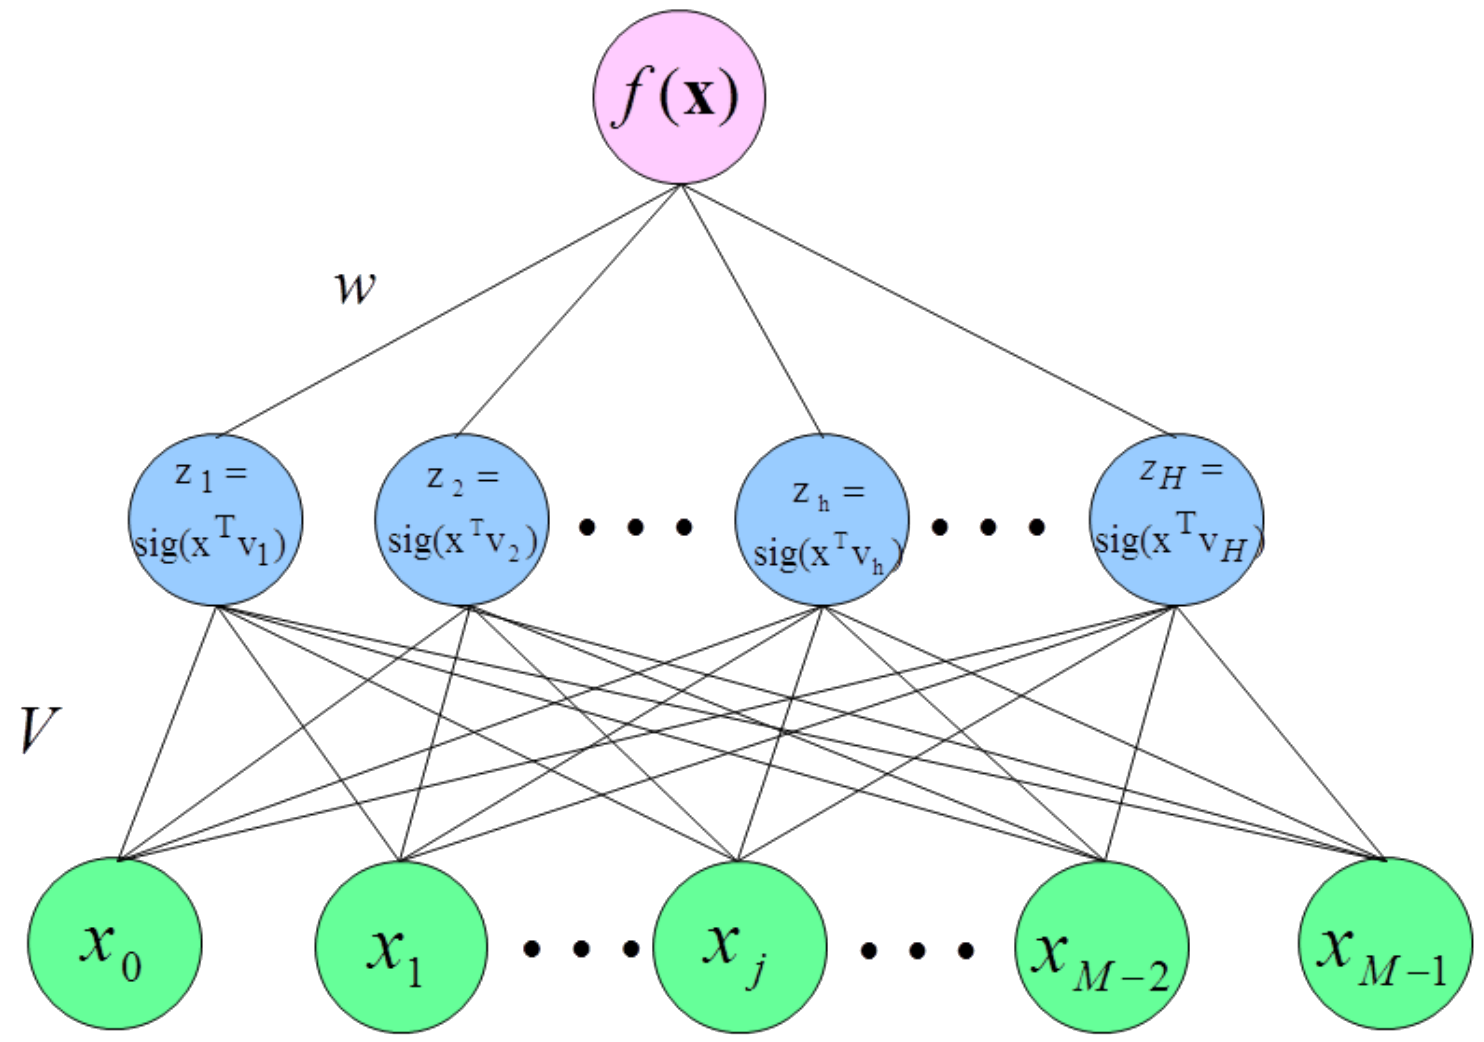
\includegraphics[width=\textwidth,height=0.4\textheight,keepaspectratio]{{{../res/Design of an artificial neural network}}}
	\caption{Design of an artificial neural network with one layer, $\pmb{x}$ as input, $z_i$ as activation function, $V$ und $w$ as weights and $f(\pmb{x})$ as prediction. Taken from~\cite{MachineLearning:NeuralNetworks}.}
	\label{fig:sample_neural_network_design}
\end{figure}

A rather simple feed-forward network is depicted in \autoref{fig:sample_neural_network_design}. Each line between two bubbles represents a connection, meaning the output of the bubble at the bottom is passed to the bubble at the top. The function used in calculating the various values for $z_i$ is called sigmoid (see~\cite{MachineLearning:NeuralNetworks}) and has an S-like shape. In terms of biology it can be though of as a boundary which has to be overcome prior to a signal being passed on. The references in the following paragraph are in regards to this figure.

Layers not representing the input or output are called hidden layers ({\color{blue}blue bubbles}). However the dimensions of an input ({\color{green}green bubbles}) are also referred to as features. The function of a node is called \textit{activation function} ($z_i$). The term \textit{learning} in the context of neural network refers to the process of adapting parameters or \textit{weights} ($V$ and $w$) of a nodes via a gradient which optimizes the desired function. The desired function is usually referred to as \textit{loss} and e.g. describes how many false classifications have been made. It is the job of the \textit{optimizer} to adapt the weights in a way which minimizes the function, a task usually done via propagating the error back through the network in a schema called \textit{back propagation}. The term \textit{training} refers to the process of applying the network to a set of data and adjusting the weights as necessary for each iteration. How many individual data points one of those iterations contains is described by the \textit{batch size}.
